\section{Problem Definition}

\begin{figure}[t]
  \centering
  \begin{subfigure}[b]{0.3\textwidth}
    \label{fig:plan_at_t0}
    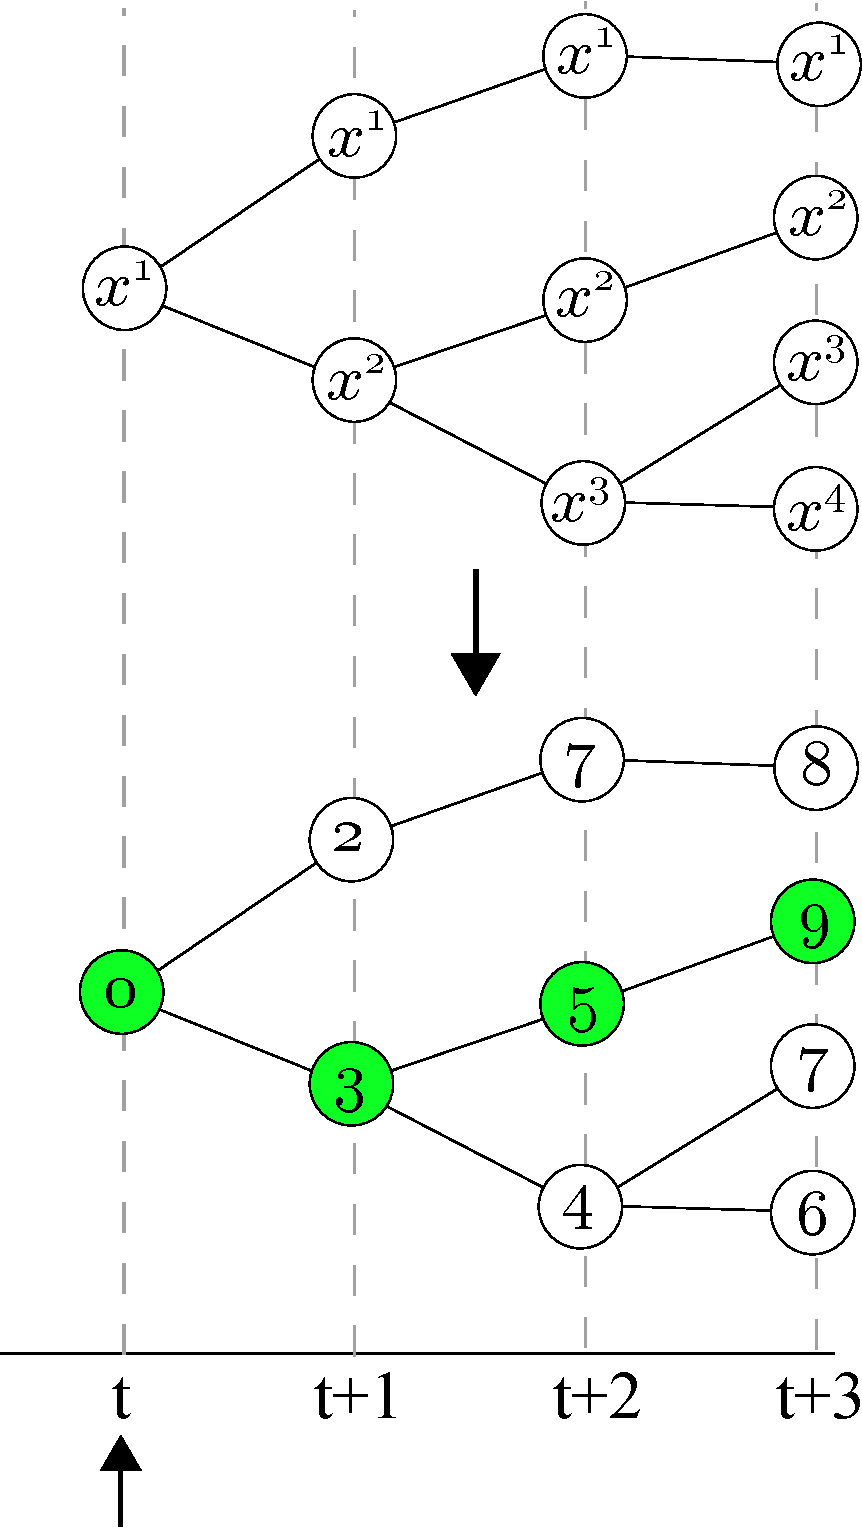
\includegraphics[height=3in]{plan_at_t0}
    \caption{}
  \end{subfigure}
  \hspace{1in}
  \begin{subfigure}[b]{0.3\textwidth}
    \label{fig:plan_at_t1}
    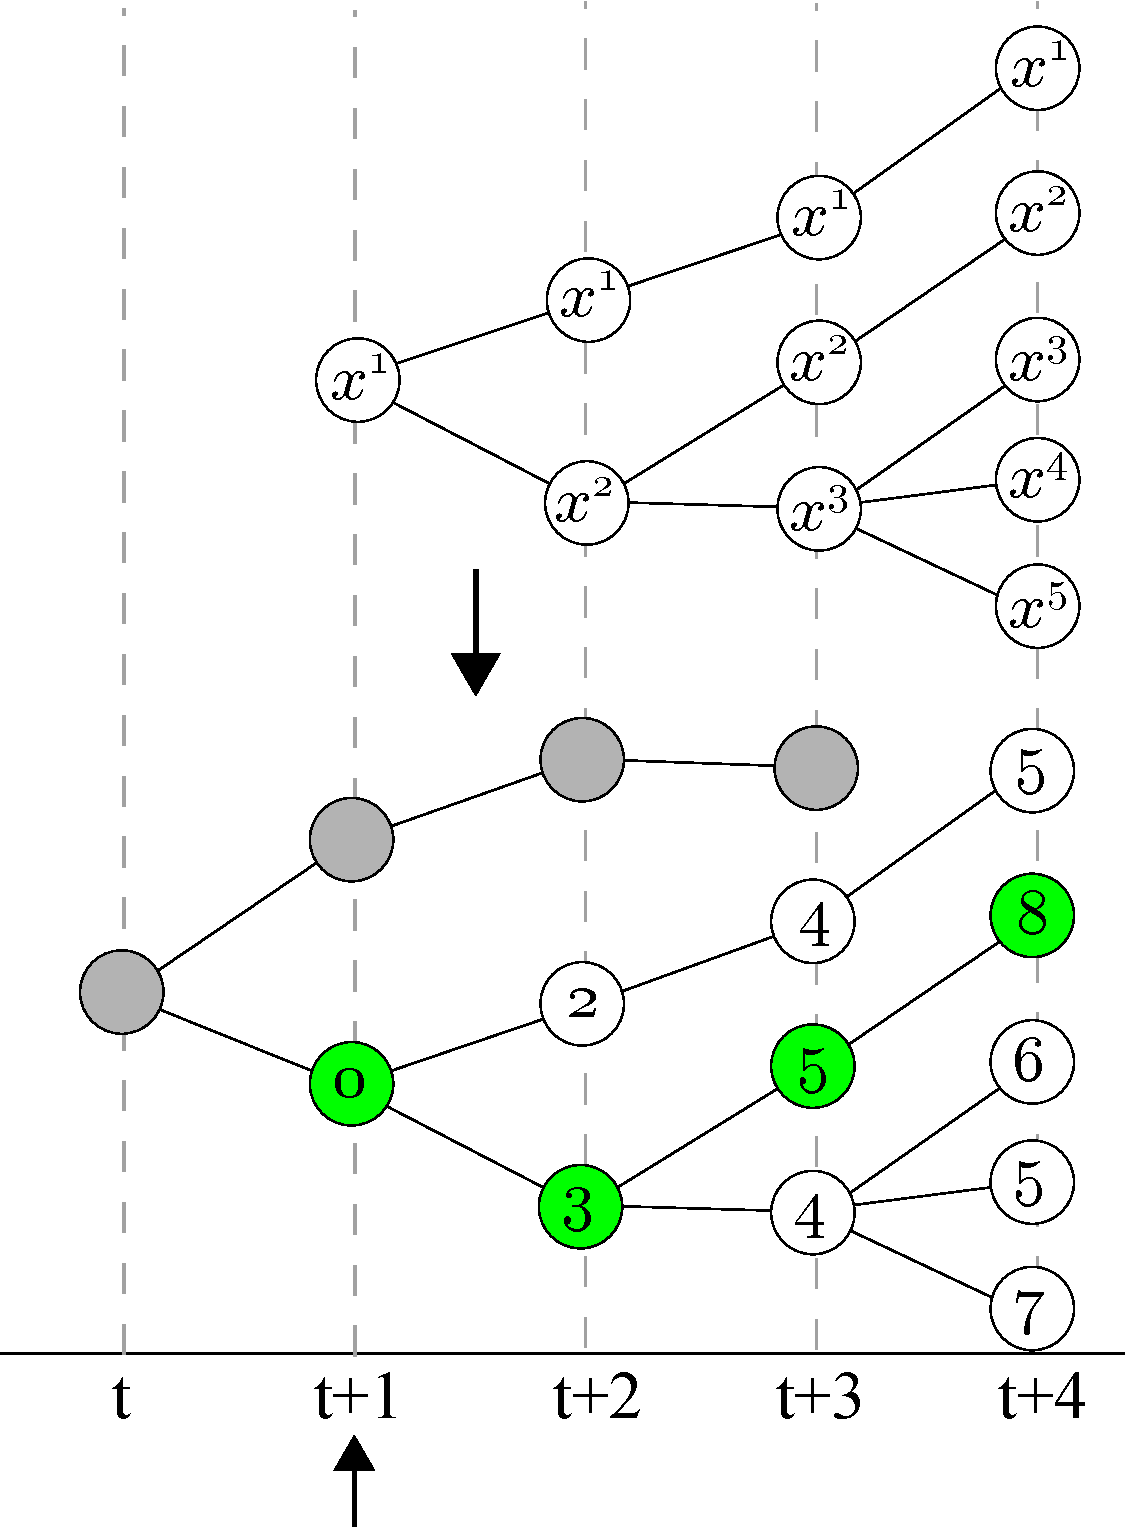
\includegraphics[height=3in]{plan_at_t1}
    \caption{}
  \end{subfigure}
  \caption{Planning trees (top) and expected mutual information trees (bottom) at times $t$ (a) and $t+1$ (b) over a 3-step horizon. As the robot moves forward, new nodes are added to the planning tree, the expected mutual information is updated based on the new sensor measurement, and the plan is refined. \label{fig:plan}}
\end{figure}


The active SLAM exploration problem can be framed as determining the control actions which guide a robot to a state that maximizes mutual information between its current and future maps. For this project, we will model the environment as an occupancy grid map, and represent the map as a conglomeration of cells: $m = \{m^{i}\}_{i=1}^{N}$. The probability that an individual cell is occupied at $t$ is given by $p\left(m^{i} \ \vert \ x_{1:t}, z_{1:t}\right)$, where $x_{1:t}$ denotes the history of states of the vehicle, and $z_{1:t}$ denotes the history of range observations accumulated by the vehicle. Additionally we assume that cell occupancies  are independent of one another: $p\left(m \ \vert \ x_{1:t}, z_{1:t}\right) = \prod_{i} p\left(m^{i} \ \vert \ x_{1:t}, z_{1:t}\right)$. For notational simplicity we write the map conditioned on random variables $x_{1:t}$ and $z_{1:t}$ as $p\left(m_{t}\right) \equiv p\left(m \ \vert \ x_{1:t}, z_{1:t}\right)$.

The optimal plan over a one step horizon will guide the robot to a state, $x_{t+1}^{*}$, in which the mutual information between $m_{t}$ and $m_{t+1}$ is maximized.

\begin{align} \begin{split}
    x_{t+1}^{*}
    &=
    \argmax_{x_{t+1}}
    \
    \text{IG}\left[
        m_{t}
        ;
        m_{t+1}
    \right]
    \\
    &=
    \argmax_{x_{t+1}}
    \
    \text{H}\left[
        m_{t}
    \right]
    -
    \expect_{z_{t+1}}\left[
        \text{H}\left[
            m_{t+1}
        \right]
    \right]
    \\
    &=
    \argmin_{x_{t+1}}
    \
    \expect_{z_{t+1}}\left[
        \text{H}\left[
            m_{t+1}
        \right]
    \right]
\end{split}
\label{eq:only_eq}
\end{align}

This is the formulation for a single step horizon, which is computed by sampling laser scans from the future state, updating the occupancy grid accordingly, and estimating the entropy of the resulting map. The goal of our project is to compute the optimal plan over multiple step horizons, which is simply an expansion of Eq.~\eqref{eq:only_eq}. We expect to be able to leverage recursive update rules to store and update expected information gain by propagating new information down a mutual information tree (Fig. \ref{fig:plan}).
